\begin{figure}
\centering
\begin{minipage}{0.4\linewidth}
    \centering
\begin{tikzpicture}

    \begin{axis}[
        ylabel={$h _{ss}$ [\%]},
        xlabel={$x$ [\%]},
        legend pos=north west,  % Position of the legend
        legend cell align={left},
        xmin=0.0,
        ymin=0.006875,
        xmax=100,
        ymax=100,
        legend pos=north east,
        xtick distance = 20,
        ytick distance = 10
    ]
    \addplot[blue] table [x expr=\thisrow{apertura}*100/(1 - 0.05) - 100*0.05/(1 - 0.05), y expr=\thisrow{nivel}*100/(30 - 0.068672) - 100*0.068672/(30 - 0.068672)]{figs/test.txt};
    \addplot[black, thick] table [x expr=\thisrow{apertura}*100/(1 - 0.05) - 100*0.05/(1 - 0.05), y expr=\thisrow{nivel}*100/(30 - 0.068672) - 100*0.068672/(30 - 0.068672)]{figs/modelo.txt};

    \node(p1) at (axis cs:15,50) [above] {$P_1(s)$};
    \node(p2) at (axis cs:8,25) [right] {$P_2(s)$};
    \node(p3) at (axis cs:20,10) [right] {$P_3(s)$};
    \node(p4) at (axis cs:50,10) [right] {$P_4(s)$};

\end{axis}
\end{tikzpicture}
\caption*{(a): Modelos dinámicos necesarios para el modelado del sistema}
\end{minipage}
\begin{minipage}{0.4\linewidth}
    \centering 
    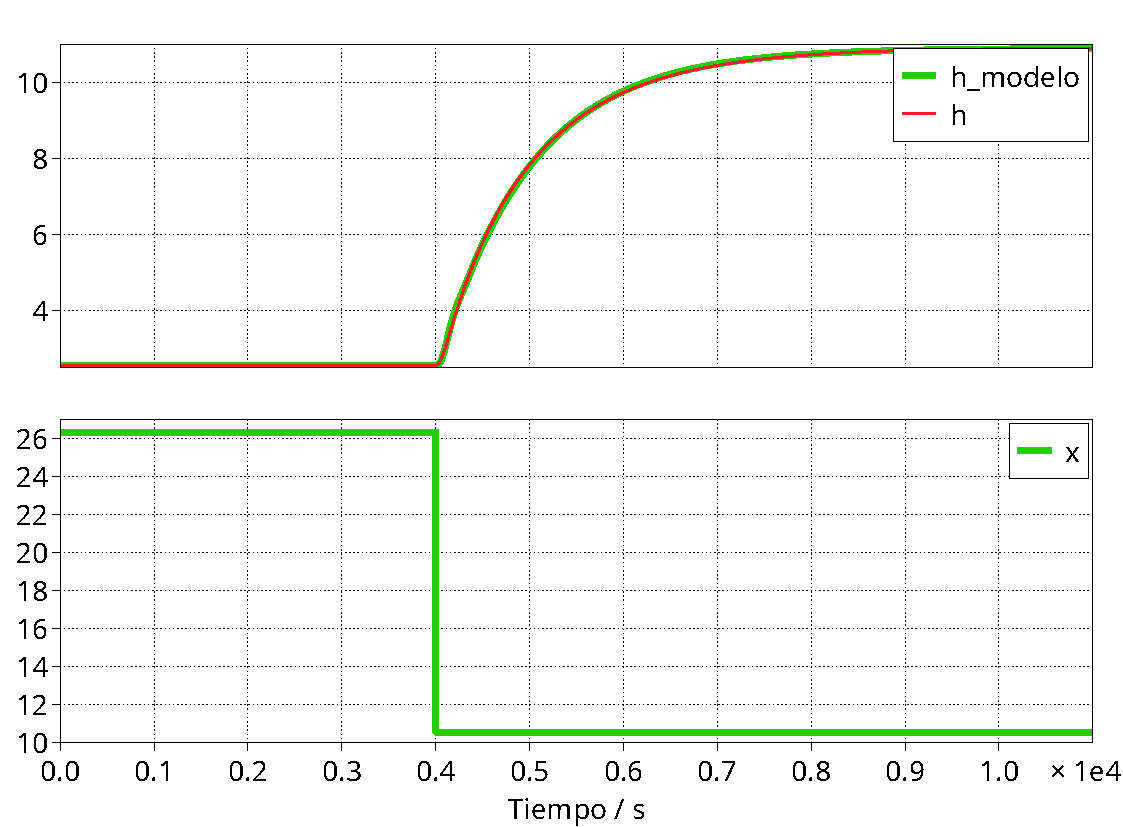
\includegraphics[width=\linewidth]{figs/scope.pdf}
    \caption*{(b): Validación del modelo identificado}
\end{minipage}
\caption{Identificación de modelos dinámicos para modelar el conjunto actuador--planta--sensor}
\label{dinamico}
\end{figure}
